\documentclass[UTF8,12pt]{ctexart}
\usepackage{amsthm}
\usepackage{amsfonts,amsmath,bm}
\usepackage{graphicx}
\usepackage{xcolor}
\usepackage{geometry}

\newenvironment{myquote}
{\begin{quote}\kaishu\zihao{5}}
{\end{quote}}

\newtheorem{definition}{定义} 
\newtheorem{theorem}{定理}

\geometry{a4paper,scale=0.8}

\begin{document}
\title{随机矩阵理论概述及其在机器学习领域中的应用 \\ \large {————独立学习总结报告}}
\author{刘书豪 20307110229}
\date{}
\maketitle

报告主要针对本学期阅读教材《Random Matrix Methods for Machine Learning》\cite{couillet_liao_2022}和《Application Of Random Matrix Theory In Statistics And Machine Learning》\cite{random2}以及
其他相关论文后所掌握的知识脉络进行梳理。本文将从结式、$Stieltjes$变换等基础工具讲起,再介绍著名的Marcenko-Pastur分布律和wigner分布律,并结合$\gamma$变换、Spiked模型等工具对一些具体的应用案例进行分析。

\tableofcontents

\newpage

\section{传统机器学习中存在的问题}

在传统机器学习研究中,我们通常需要做一个重要假设,即数据的样本-特征比是足够大的。
在这一假设下,我们可以借助大数定理、中心极限定理等传统概率论工具来解释实验结果的可靠性。

但在如今的大数据时代,很多时候不仅样本量很大,特征数量也十分庞大,例如无线信号传输领域的\cite{Li2007MIMORW}、金融统计领域\cite{Laloux2000RANDOMMT}中都会出现维度很高的数据。在这种情况下,传统的大数定律
和中心极限定律都会失效,一些传统认知下的共识也会发生变化\cite{vaart_1998}。这里有两个简单的例子:

1、相关系数矩阵不收敛。

\begin{myquote}
    假设由一组服从标准高斯分布的数据(共1000条),
    先假设数据维数为10的样本,即样本矩阵大小为$1000 \times 10 $,
    此时关于维度的协方差矩阵是一个$10\times 10$的矩阵,且根据强大数定律,该相关系数矩阵是几乎处处
    收敛到单位矩阵的。
    若假设样本的维数是2000,此时得到的相关系数矩阵为$2000\times 2000$的矩阵,但它的秩最多不超过
    1000,故不可能收敛到单位矩阵。
\end{myquote}

2、欧式度量“失效”
\begin{myquote}
    考虑两组均值为0,标准差一大一小(但是均为$O(1)$量级)的高斯分布样本。在低维空间中,明显高标准差样本会集中分布在
    离原点更远的地方;但是在高维空间中,假设空间维度为$p$十分大,可以证明样本的范数$\Vert x\Vert\sim O(\sqrt{p})$,但$\Vert x\Vert-E[\Vert x\Vert]
    \sim O(1)$,即两组样本的主要信息都被维度$p$盖住了,这时候再用低维时的方法去处理问题就会失效了。
\end{myquote}

总之,我们需要找到更准确的数学语言去刻画这种模型。

例如,涉及以下两个方面的问题可以借助随机矩阵的工具,在样本数并未远远大于特征数的情况时,得到更准确的结果:

\begin{itemize}
    \item 协方差矩阵,如主成分分析 (PCA)、线性判别分析 (LDA)等。
    \item 核矩阵,主要运用于各种核方法。
\end{itemize}
我们将在最后给出这两个方向的应用案例。

\section{随机矩阵理论}

在随机矩阵的研究历史上,一开始人们将目光放在对一个确定维数的随机矩阵经验谱分布的精确刻画上,但这样不仅只有
极少的特殊分布可以计算出精确值,而且得到的结果也十分复杂\cite{Wishart1928THEGP}。之后一部分学者便将目光转向了
渐近随机矩阵——即假设样本矩阵的样本数$n$和维数$p$在以下渐进条件下:
\[
    \lim\limits_{n,p \rightarrow \infty}\frac{p}{n} = c \in (0,\infty),
\]  

在这一渐进框架下,我们也有很多不同的工具来解决问题,例如矩方法\cite{Wigner1955CharacteristicVO}、自由概率理论\cite{Voiculescu1992FreeRV}等
。本节将主要介绍另一种工具——Stieltjes变换,它类似于随机变量的Fourier变换(特征函数),给予了我们一个方便的途径去刻画矩阵的经验谱分布。
\subsection{基础工具}

\begin{definition}
    对于一个n维实对称方阵$M$,记其谱为$\sigma(M)$,则$M$的\textbf{结式}为一个矩阵函数:
    \begin{equation*}
        \begin{aligned}
            Q_M(z):  \quad & \mathbb C \backslash \sigma(M) \rightarrow \mathbb C^{n\times n} \\
                    & z \rightarrow {(M-zI_n)}^{-1}. \\
        \end{aligned}
    \end{equation*}
 
\end{definition}

\begin{definition}
    对于一个n维实对称方阵$M$,记其谱为$\sigma(M)$,则$M$的\textbf{经验谱分布}$\mu_M$为:

    \begin{equation*}
        \mu_M = \frac{1}{n}\sum\limits_{\lambda \in \sigma(M)} \delta_{\lambda},
    \end{equation*}
 
    其中$\delta_{\lambda}$为$\lambda$的计数测度。
\end{definition}

\begin{definition}
    对于一个实值测度$\mu$,它的\textbf{Stieltjes变换}是一个定义在$\mathbb C \backslash \textup{supp}(\mu) $上
    的函数:
    \[
    m_{\mu}(z) = \int \frac{1}{t-z}\mu(dt).
    \]
\end{definition}

类似于Fourier变换,Stieltjes变换也具有许多比较好的性质,如:
\begin{itemize}
    \item 它在定义域上是复解析的。
    \item 它是有界的,$|m_{\mu}(z)| \leq \frac{1}{dist(z,\textup{supp}(\mu))}$,其中dist表示(点到集合的)欧式度量。
    \item $\Im[z]>0$ 蕴含着 $\Im[m_{\mu}(z)]>0$。
    \item 如果将其限制在$\mathbb R$上,在每个连通分支上它是单调递增的
    ,且$\lim\limits_{x \rightarrow \pm \infty} m_{\mu}(x)= 0$。
\end{itemize}

当然,最重要的还是它的逆转公式:

\begin{theorem}
    对于一个概率测度$\mu$,任取$a,b$为它的两个连续点,则我们有:
    \[
        \mu([a,b]) = \frac{1}{\pi} \lim\limits_{y \downarrow 0} \int_a^b \Im[m_{\mu}(x+iy)]dx,   
    \]
    进一步,如果$\mu$在x点具有密度函数$f$,则:
    \[
        f(x) = \frac{1}{\pi}\lim\limits_{y \downarrow 0}\Im[m_{\mu}(x+iy)],
    \]
    同时,如果$\mu$在x点有离散分布,则:
    \[
        \mu({x}) = \lim\limits_{y\downarrow 0}-iym_{\mu}(x+iy).  
    \]
\end{theorem}

更重要的是,如果这里的测度是经验谱分布,则我们有(记$M$的特征值一共有$n$个):

\[
    m_{\mu_M}(z) = \frac{1}{n}\sum\limits_{\lambda \in \sigma(M)}\int\frac{\delta_{\lambda}(t)}{t-z}
    = \frac{1}{n}\sum\limits_{\lambda \in \sigma(M)}\frac{1}{\lambda-z} = \frac{1}{n}trQ_M(z).
\]

可以看到,我们将经验谱分布的Stieltjes变换和结式联系起来了,同时Stieltjes的逆转公式又天然地
告诉了我们经验谱分布的分布函数,故我们只需要研究矩阵的结式就可以知道其经验谱分布。

在本节结尾再介绍两个概念,它会使得我们在后续描述定理的时候更加方便:

\begin{definition}
    对于两个n维的随机矩阵或确定矩阵$X,Y$,我们称它们\textbf{确定性等价},如果任取
    (算子函数意义下的)有界矩阵
    $A$和有界向量$a,b$,在几乎处处或者依概率意义下有:

    \[
        \frac{1}{n}trA(X-Y)\rightarrow 0, \quad a^T(X-Y)b \rightarrow 0, \quad
        \Vert\mathbb E[X-Y]\Vert \rightarrow 0, \quad n \rightarrow \infty,
    \]
    此时我们记作 $X\leftrightarrow Y$.
\end{definition}

\begin{definition}
    记$\mathcal{A}$为$\mathbb C$的一个子集,$m \in \mathbb C, z \in \mathcal{A}$,则我们称
    \[
        \{(z,m)\in\mathcal A \times \mathbb C \;|\; 
        (\Im[z]\neq 0 \;\text{且} \; \Im [z] \cdot \Im[m]>0) \;\text{或}\; 
    \]
    \[
        (m>0 \;\text{且}\; z < \inf \mathcal A^C \cap \mathbb R) \;\text{或}\; 
        (m<0 \;\text{且}\; z>\sup\mathcal A^C \cap \mathbb R) \}  
    \]
    为$\mathcal A$的Stieltjes对集合,并记之为$\mathcal Z (\mathcal A)$.
\end{definition}

Stieltjes对的定义是为了方便确定合理的Stieltjes变换(
后文的$m(z)$可能是通过解一个具有多个根的方程得到的,故可能会产生没有意义的根),
这是因为在之前的性质我们提到过$\Im [z] \cdot \Im[m]>0$。
后两种情况是对$\Im[z] = 0$的补充。

\subsection{MP分布律、Wigner半圆分布律及其推广}

本节主要介绍随机矩阵理论中最经典的两大分布律。

之前提到过我们研究的框架是基于渐近假设的,
在这一假设下,Marcenko和Pastur给出了著名的MP分布律\cite{MP1}:

\begin{theorem}\label{MPLaw}
    设$X \in \mathbb R ^{p\times n}$ 为每个元素都服从均值为0且方差为1的轻尾分布的随机矩阵,
    记$Q(z)={(\frac{1}{n}XX^T-zI_p)}^{-1}$为$\frac{1}{n}XX^T$的结式,那么当
    \[
        \lim\limits_{n,p \rightarrow \infty}\frac{p}{n} = c \in (0,\infty),
    \]  
    时,我们有:
    \[
        Q(z) \leftrightarrow \bar{Q}(z), \quad \bar{Q}(z) = m(z)I_p,
    \]
    其中$(z,m(z))$是下述方程在$\mathcal Z (\mathbb C \backslash [{(1-\sqrt{c})}^2
    ,{(1+\sqrt c)}^2])$内的\textbf{唯一}解:
    \[
        zcm^2(z)-(1-c-z)m(z)+1 = 0,
    \]  
    进一步地,使用逆转公式可以得到$m(z)$为以下概率测度的Stieltjes变换:
    \[
        \mu(dx) = {(1-c^{-1})}^+ \delta_0(x) + \frac{1}{2\pi cx}\sqrt{
            {(x-E_-)}^+ {(E_+ -x)}^+
        }dx,
    \]
    其中$E_{\pm} = {(1\pm\sqrt{c})}^2, {(x)}^+ = \max(0,x)$,且我们称$\mu$为Marcenko-Pastur分布。
    
最关键地,矩阵$\frac{1}{n}XX^T$的经验谱分布$\mu_{\frac{1}{n}XX^T}$在上述渐近规律下弱收敛到$\mu$。
\end{theorem}

在$c$取不同值时的MP分布如下图所示(图片摘自\cite{couillet_liao_2022}P52,Figure\,2.2):

\begin{figure}[htbp]
    \centering
    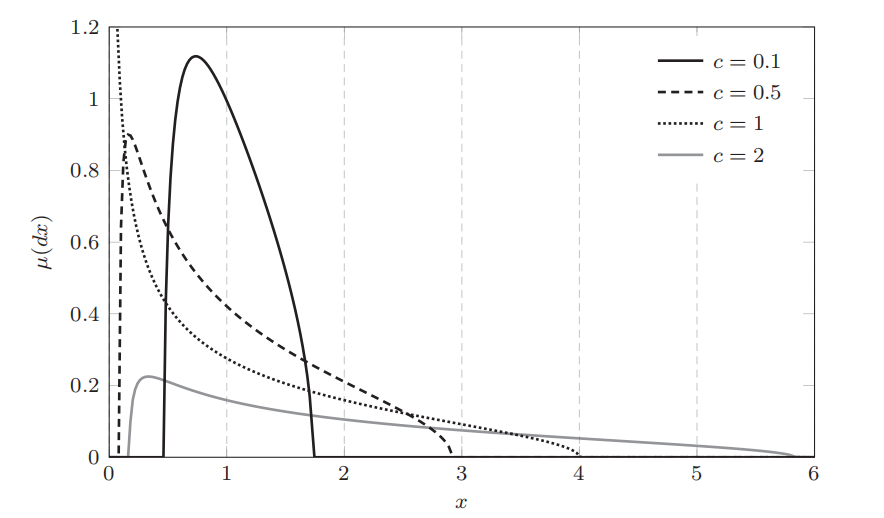
\includegraphics[width=1\textwidth]{MP_law.png}
\end{figure}

上述定理的证明是繁琐的,这里仅对证明思路进行介绍:
\begin{itemize}
    \item[(1)] 由于$Q$是对称阵,故可以进行谱分解,记$Q_{-1}$为丢掉第一个谱之后的矩阵
    (即若$Q = \sum\limits_{k=1}^n v_k {v_k}^T$为Q的谱分解,则$Q_{-1} = \sum\limits_{k=2}^n v_k {v_k}^T$),
    定义中间变量:
    \[
        \alpha (z) = \frac{1}{n} tr \mathbb E (Q_{-1}(z)),\quad \bar{\bar{Q}}(z) = 
        {(-z + \frac{1}{1+\alpha(z)})}^{-1}I_p   , 
    \]
    然后证明$\Vert\mathbb Q [Q - \bar{\bar{Q}}]\Vert \sim O(n^{-\frac{1}{4}})$.
    \item[(2)] 再证明$|\alpha(z) - cm(z)| \rightarrow 0$,进而得到$\Vert\bar Q(z) - \bar{\bar Q}(z)\Vert \rightarrow 0$.
    进而得到确定等价的第三个关系$\Vert\mathbb E [Q(z)-\bar Q(z)]\Vert\rightarrow 0$.
    \item[(3)] 最后再证明$\frac{1}{p} tr A(Q-\bar Q) \rightarrow 0, a^T(Q-\bar Q)b \rightarrow 0$即可。
    \item[(4)] 根据上述结果,类似于特征函数可证弱收敛性。 
\end{itemize}

MP法则自然的可以应用到协方差矩阵上。

\begin{itemize}
    \item MP律的应用条件十分广泛,只需要分布是一个轻尾分布就可以使用。(实际上轻尾分布的条件也过强了,根据证明过程,只需要该分布具有8阶以上的有限矩就可以证明MP律,
    这里只写轻尾分布主要是因为在后续推广定理证明中,如果只要求8阶有限矩,可能不一定够用)。
    \item 代入数据计算可以发现,尽管c的值达到$\frac{1}{100}$,其经验谱分布在渐近意义下相较于$I_n$也有将近0.2的误差。
\end{itemize}

上述定理是最基本的形式,事实上还有许多变式,这里不再详细阐述,只给出一个应用范围最广的推广\cite{MP2},即考虑数据各个维度间具有线性相关性的情形:

\begin{theorem}\label{MP2}
    若$X = C^{\frac{1}{2}}Z$,其中C为一个半正定矩阵表示协方差矩阵,
    $Z \in \mathbb R ^{p\times n}$ 为每个元素都服从均值为0且方差为1的某轻尾分布的随机矩阵,
    并且定义$Q(z)={(\frac{1}{n}XX^T-zI_p)}^{-1}, \tilde Q(z) = {(\frac{1}{n}X^T X-zI_n)}^{-1}$,则有:
    \[
        Q(z) \leftrightarrow \bar{Q}(z) = -\frac{1}{z}{(I_p + \tilde{m}_p(z)C)}^{-1}, 
    \]
    \[
        \tilde Q(z) \leftrightarrow \bar{\tilde{Q}} = \tilde{m}_p(z)I_n,
    \]  
    其中$(z,\tilde{m}_p(z))$为下述方程在$\mathcal Z (\mathbb C \backslash \mathbb R^+)$内的\textbf{唯一}解:
    \[
        \tilde{m}_p(z) = {(
            -z + \frac{1}{n}trC{(I_p + \tilde{m}_p(z)C)}^{-1}
        )}^{-1},
    \]  
    特别的,如果C的经验谱分布收敛到某一分布$\nu (p \rightarrow \infty)$,则有
    \[
        \mu_{\frac{1}{n}XX^T} \stackrel{a.s.}{\rightarrow} \mu,\quad \mu_{\frac{1}{n}X^T X} \stackrel{a.s.}{\rightarrow} \tilde \mu,
    \]
        其中$\mu,\tilde\mu$的Stieltjes变化恰好为$m(z)$和$\tilde m (z)$,且:
    \[
        m(z) = \frac{1}{c}\tilde m(z) + \frac{1-c}{cz},\quad
        \tilde m(z) = {(
            -z + c\int\frac{t \nu (dt)}{1+\tilde m (z)t}
        )}^{-1}.
    \]
\end{theorem}

从定理\ref{MP2}中可以看出实际上协方差矩阵和Gram矩阵的经验谱分布是息息相关的,如果将样本看成时间,特征看成空间,
我们可以说MP律反映了时空之间的联系。这一观点在其他的推广中显得极为重要(如$C^{\frac{1}{2}}Z\tilde{C}^{\frac{1}{2}}$形式的矩阵)。

但这样也带来一个问题,便是如何计算出准确值,想要求出精确的解析解就必须得保证分布$\nu$具有较好的形式。
一般地,我们可以通过迭代的数值方法进行求解\cite{numericalMP}:
\[
    m^{(l)}(z) = \frac{1}{c}\tilde m^{(l)}(z) + \frac{1-c}{cz},\quad
    \tilde m^{(l+1)}(z) = {(
        -z + c\int\frac{t \nu (dt)}{1+\tilde m^{(l)} (z)t}
    )}^{-1},
\]
该方法的收敛性已被证明。

注:在运用迭代法计算时,越靠近$\textup{supp}(\mu)$的点收敛速度越慢,所以常用的处理手法为先计算远离$\textup{supp}(\mu)$的点的数值,再逐步往靠近
$\textup{supp}(\mu)$计算,这样每次迭代的初值可以尽可能的接近准确值,进而加快迭代速度。

在本节的最后简单叙述一下经典的Wiger半圆分布律定理\cite{wigner}。

\begin{theorem}
    记$X \in \mathbb R^{n \times n}$为一个对称随机矩阵,其中每个元素都服从某均值为0方差为1的轻尾分布,
    记$Q(z) = {(
        \frac{X}{\sqrt{n}}-zI_n
    )}^{-1}$,则当$n \rightarrow \infty$时,我们有:
    \[
        Q(z) \leftrightarrow \bar Q(z) = m(z)I_n,  
    \]
    其中$(z,m(z))$为下述方程在$\mathcal Z (\mathbb C \backslash [-2,2])$内的\textbf{唯一}解:
    \[
        m^2(z) +zm(z) + 1 = 0,
    \]
    且经计算可得$m(z)$为下述概率分布的Stieltjes变换:
    \[
        \mu(dx) = \frac{1}{2\pi}\sqrt{
            {(4-x^2)}^+
        }dx.
    \] 
    我们称该分布为Wigner半圆分布。
\end{theorem}

\subsection{关于协方差矩阵经验谱分布的进一步讨论}
本节的所有讨论都将基于定理\ref{MP2}的条件。事实上,它和定理\ref{MPLaw}是一致的,因为$I_n$的经验谱分布测度$\nu$就是$\delta_1$。

在定理\ref{MP2}中我们得到了$\frac{1}{n}XX^T$和$\frac{1}{n}X^T X$的极限经验谱分布$\mu$和$\tilde \mu$
,根据高代的知识不难知道$\mu = \frac{1}{c}\tilde\mu + (1-\frac{1}{c})\delta_0$,故我们只需将目光集中到$\tilde\mu$的求解上。

只考虑$\tilde \mu$的好处在于我们有以下关系式:
\begin{equation}\label{m}
    \tilde m(z) = {(
        -z + c\int\frac{t \nu (dt)}{1+\tilde m (z)t}
    )}^{-1},
\end{equation}
它和$m(z)$无关。

\subsubsection{利用Stieltjes变换的反函数求解$\textup{supp}(\tilde\mu)$}

直接求解方程 (\ref{m}) 来得到$\tilde m$的精确值是难以操作的,但我们可以将其变形为:

\begin{equation}\label{inverse}
    z = -\frac{1}{\tilde m(z)} + c \int \frac{t \nu (dt)}{1+t\tilde m(z)}.
\end{equation}

这样我们得到了一个定义在$\tilde m (\mathbb C \backslash \textup{supp}(\tilde \mu))$上的Stieltjes变换的逆
(如果只从函数本身的良定出发,定义域可以
拓展到$\{\tilde m \in \mathbb C | 0 \notin 1 + \tilde m \cdot \textup{supp}(\nu)\}$上),但我们更关心该函数限制在$\mathbb R$
上的取值,这有以下几点好处:

\begin{itemize}
    \item 只考虑在实轴上的取值就已经足够得到$\tilde\mu$的相关信息了,而且还利于结果的可视化。
    \item 在$\mathbb R \backslash \textup{supp}(\tilde\mu)$上,Stieltjes变换是单调递增的,故其反函数也应该是单调递增的,
    进一步的,Silverstein和Choi也证明了反函数的每一段单调递增区间也对应了Stieltjes变换的一段逆。
    \item 和上面提到的一样,定义域是可以拓展到$\{\tilde m \in \mathbb R | 0 \notin 1 + \tilde m \cdot \textup{supp}(\nu)\}$上
    的,为了区分,我们记这段上的“Stieltjes变换”为$\tilde m ^\circ (z)$,可以证明,$\tilde m ^\circ (z) = \lim\limits_{\epsilon \downarrow 0}\tilde m (x+i\epsilon)$是存在的,
    进而根据关系式$\Im[z]\cdot\Im[m(z)]>0$和控制收敛定理可以知道$\tilde m ^\circ (z)$为下述方程的正虚部解:
    \[
        \tilde m^\circ(z) = {(
            -z + c\int\frac{t \nu (dt)}{1+\tilde m^\circ (z)t}
        )}^{-1} ,
    \]  
    解的唯一性也已被证明。此时再配合逆转公式便可得到$\tilde \mu$在$\textup{supp}(\tilde \mu)$上的概率密度函数。
\end{itemize}

总结一下,我们实际上得到了以下定理\cite{solve}:

\begin{theorem}
    在定理\ref{MP2}的假设下,如果我们定义以下函数:
    \begin{equation*}
        \begin{aligned}[]
            x(\cdot): && \mathbb R \backslash \{\tilde m| -\frac{1}{\tilde m} \in \textup{supp}(\nu)\} & \rightarrow \mathbb R \\
            && \tilde m & \rightarrow -\frac{1}{\tilde m} + c \int \frac{t \nu(dt)}{1+t\tilde m}, \\
        \end{aligned}    
    \end{equation*}

    则$\tilde \mu$在$\mathbb R \backslash \{0\}$上具有概率密度函数,且

    \begin{itemize}
        \item $\textup{supp}(\tilde \mu) \backslash \{0\} = \mathbb R \backslash \{
            x(\tilde m) | -\frac{1}{\tilde m}\in \mathbb R \backslash \{\textup{supp}(\nu)\cup \{0\}\}\;\text{且}\;x^{\prime}(\tilde m)>0  
        \}$.
        \item $\forall y \in \textup{supp}(\tilde\mu), \tilde \mu (dy) =
        \begin{cases}
            \frac{1}{\pi}\Im[\tilde m^{\circ}(y)] & y \neq 0 \\
            -iy\tilde m^{\circ}(y) & y = 0 \\
        \end{cases}
        $,其中$\tilde m^{\circ}(y)$为方程$x(\tilde m^{\circ}(y)) = y$的唯一正虚部解。
    \end{itemize}
\end{theorem}

\subsubsection{$\textup{supp}(\nu)$和$\textup{supp}(\mu)$的关系}

我们定义一个变量代换函数:

\begin{equation*}
    \begin{aligned}
        \gamma: && \mathbb C \backslash \{\textup{supp}((\mu)) \cup \{0\} \} & \rightarrow \mathbb C \\
        && z = z(\tilde m) & \rightarrow -\frac{1}{\tilde m},\\
    \end{aligned}
\end{equation*}

不难证明$\gamma$是一个单射且具有以下良好性质:
\[
    \gamma(
        \mathbb C \backslash \mathbb R
        ) \subset \mathbb C \backslash \mathbb R 
        \quad \text{且} \quad 
        \gamma(
        \mathbb R \backslash \textup{supp}(\mu)
    ) \subset \mathbb R \backslash \textup{supp}(\nu).
\]  

映射$\gamma$的单射性保证了其能把复平面内的一条闭曲线映为另一条闭曲线而且反之(局部上)也能映射回来,同时另一条性质也保证了映射前后$\textup{supp}(\mu)$和$\textup{supp}(\nu)$都被包含在了
曲线内部,配合Cauchy积分公式,这一点将在后面的统计推断中起到关键作用。

下图清楚展示了映射$\gamma$的作用效果(图片摘自\cite{couillet_liao_2022}P85,Figure\,2.6):

\begin{figure}[htbp]
    \centering
    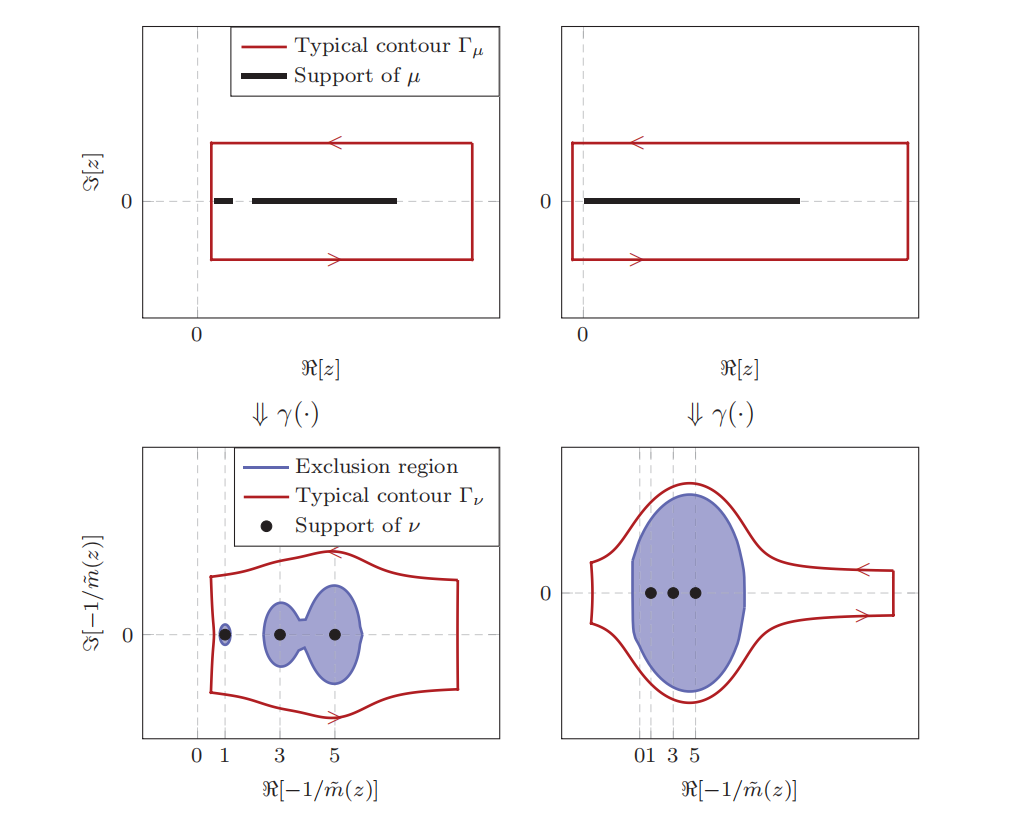
\includegraphics[width = 1\textwidth]{gamma.png}
\end{figure}

将$\textup{supp}(\nu)$和$\textup{supp}(\mu)$联系起来还有一个好处。如果只考虑$\textup{supp}(\mu)$,定理\ref{MP2}中的弱收敛性
实际上只能告诉我们,任取有界连续函数$f$,我们有
\[
    \frac{1}{p} \sum\limits_{i=1}^{p}f(\lambda_i(
        \frac{1}{n}XX^T
    )) - \int f(t)\mu(dt) \stackrel{a.s.}{\longrightarrow} 0.
\]  

此时如果在上式中取$f$为特征函数$1_{[a,b]}$的光滑化函数,其中$[a,b] \subset \mathbb R \backslash \textup{supp}(\mu)$,
只能得到$[a,b]$内$\frac{1}{n}XX^T$特征值个数的数量级为$o(p)$而不是$o(1)$,即特征值很可能会发生“泄露”!

不过Bai和Silverstein一起在1988年和1998年借助$\gamma$变换分别给出了这一问题在两种不同情况下的解答\cite{gamma2}\cite{gamma1},我们仅将定理陈述如下:

\begin{theorem}
    在定理\ref{MP2}的假设下,如果$C$在算子范数意义下有界,且
    \[
        \max\limits_{1 \leq i \leq p} dist(\lambda_i(C), \textup{supp}(\nu)) \rightarrow 0,
        \quad p \rightarrow \infty,
    \]

    则任取$0 \leq a < b \leq \infty$且$a,b \notin \textup{supp}(\mu)$,我们有:
    \begin{itemize}
        \item 若$\mathbb E[|Z_{ij}|^4] < \infty$,则:
        \[
            \#\{
                \lambda_i(\frac{1}{n}XX^T) \in [a,b]
            \}  -
            \#\{
                \lambda_i(C) \in [\gamma(a),\gamma(b)]
            \}  
            \stackrel{a.s.}{\longrightarrow} 0,
        \]
        特别地,如果$[a,b]$是$\mathbb R^+ \backslash \textup{supp}(\mu)$的一个连通子集,则有:
        \[
            \#\{
                \lambda_i(\frac{1}{n}XX^T) \in [a,b]
            \} 
            \stackrel{a.s.}{\longrightarrow} 0.
        \]
        \item 若$\mathbb E[|Z_{ij}|^4] = \infty$,则:
        \[
            \max\limits_{1 \leq i \leq p} \lambda_i(\frac{1}{n}XX^T) \stackrel{a.s.}{\longrightarrow} \infty.
        \]  
    \end{itemize}
\end{theorem}

\subsection{关于$C$特征值的统计推断}

本节中将基于$\gamma$变换阐述一个随机矩阵理论的应用案例。

当我们拿到一个样本矩阵时,如果我们假设数据的各个特征之间存在某种线性相关性(即服从定理\ref{MP2}中假设)
,则我们希望从数据出发算出$C$(或者找到相关的统计估计量),这在某种意义上可以看成是定理\ref{MP2}的“逆命题”。
本节将给出$\frac{1}{p}\sum\limits_{i=1}^p f(\lambda_i(C))$的统计估计量。

我们再次把目光放回方程 (\ref{m})。该式中的积分也可以看成是$\nu$的Stieltjes变换,即:
\begin{equation*}
    \begin{aligned}
        \int \frac{t\nu(dt)}{1+t\tilde m(z)} & = \frac{1}{\tilde m(z)} \int \frac{t \tilde m(z)\nu(dt)}{1 +t\tilde m(z)} \\
        & = \frac{1}{\tilde m(z)} (1 - \int\frac{\nu(dt)}{1+t\tilde m(z)}) \\
        & = \frac{1}{\tilde m(z)} (1 - \frac{1}{\tilde m(z)} \int \frac{\nu(dt)}{t-(-\frac{1}{\tilde m(z)})}) \\
        & = \frac{1}{\tilde m(z)}(1 - \frac{1}{\tilde m(z)} m_{\nu}(-\frac{1}{\tilde m(z)})).\\
    \end{aligned}
\end{equation*}  

再结合等式$m(z) = \frac{1}{c}\tilde m(z) + \frac{1-c}{cz}$,不难得出:
\[
    m_\nu (-\frac{1}{\tilde m(z)}) = -zm(z) \tilde m(z).
\]  

下面我们考虑相关矩阵$C$的经验谱分布$\nu$,如果我们记$\nu = \frac{1}{p}\sum\limits_{i=1}^p \delta_{\lambda_i(C)}$,则
结合Cauchy积分公式可以得到:

\begin{equation*}
    \begin{aligned}
        \frac{1}{p}\sum\limits_{i=1}^p f(\lambda_i(C)) &
        = \int f(t) \nu(dt) \\
        & = \int[\frac{1}{2\pi i} \oint_{\Gamma_{\nu}} \frac{f(z)dz}{z-t}]\nu(dt)\\
        & = -\frac{1}{2\pi i} \oint_{\Gamma_{\nu}} f(z) [\int \frac{\nu(dt)}{t-z}]dz\\
        & = -\frac{1}{2\pi i} \oint_{\Gamma_{\nu}} f(z) m_\nu(z) dz.\\
    \end{aligned}
\end{equation*}  
这里$f(\cdot)$为在$C$所有特征值邻域的某邻域上解析的函数,$\Gamma_\nu \subset \mathbb C$为一条包含$\textup{supp}(\nu)$但不包含$f(\cdot)$奇点的逆时针闭曲线。

进一步地我们考虑$\gamma$(逆)变换,则环绕$\textup{supp}(\nu)$的$\Gamma_\nu$被映为了环绕$\textup{supp}(\mu)$的$\Gamma_\mu$,且:
\begin{equation*}
    \begin{aligned}
        \frac{1}{p}\sum\limits_{i=1}^p f(\lambda_i(C)) &
        = -\frac{1}{2\pi i} \oint_{\Gamma_\mu} f(-\frac{1}{\tilde m(\omega)})m_\mu(\frac{1}{\tilde m(\omega)})\frac{{\tilde m}^\prime(\omega)}{{\tilde m}^2(\omega)}d\omega \\
        & = \frac{1}{2\pi i} \oint_{\Gamma_\mu} f(-\frac{1}{\tilde m(\omega)}) \omega \frac{m(\omega){\tilde m}^\prime(\omega)}{\tilde m (\omega)}d\omega\\
        & = \frac{1}{2c\pi i} \oint_{\Gamma_\mu} f(-\frac{1}{\tilde m(\omega)}) \omega {\tilde m}^\prime(\omega) d\omega -\frac{1-c}{c} f(0) \cdot 1_{\{ 0 \in \Gamma_\nu^\circ \}}, \\
    \end{aligned}
\end{equation*}  
其中角标$\circ$表示曲线的内部。

可以证明,在特征值不“泄露”的条件下,也即:
\[
    \max\limits_{1 \leq i \leq p} dist(\lambda_i(C), \textup{supp}(\nu)) \rightarrow 0, \mathbb E [{|Z_{ij}|}^4] < \infty,
\]  
结合复分析的相关知识,等式右边满足控制收敛定理的条件,根据定理\ref{MP2}的结论,此时我们可以用$m_{\frac{1}{n}X^T X}$代替$\tilde m$,即:
\begin{equation}\label{si}
    \frac{1}{p}\sum\limits_{i=1}^p f(\lambda_i(C)) - \frac{1}{2c\pi i} \oint_{\Gamma_\mu} f(-\frac{1}{m_{\frac{1}{n}X^T X}(\omega)}) \omega {m_{\frac{1}{n}X^T X}}^\prime(\omega) d\omega \stackrel{a.s.}{\longrightarrow} 0.
\end{equation}
这里的$\Gamma_\mu$是在右半平面中环绕$\textup{supp}(\mu) \backslash \{0\}$的闭曲线。

之所以不考虑零点是因为,我们前面关于$\gamma$变换的讨论都是限制在右半平面上的,如果是包含零点的闭曲线势必会涉及到左半平面,无法保证结果的准确性。

这也告诉我们上述近似方法最好应用于$c<1$的情形(否则0点会有原子质量),这也是符合我们的认知的——当$p>n$时,想从样本推断出相关矩阵的信息肯定是不够的。

下面我们考虑一个具体的例子。假设我们知道$C$的经验谱分布按一定比例分为有限个不同特征值,即:
\[
    \nu_C = \frac{1}{p}\sum\limits_{i=1}^{k}p_i\delta_{l_i} \rightarrow 
    \sum\limits_{i=1}^{k}c_i\delta_{l_i},
\]  
其中$l_1 > l_2 > \cdots > l_k > 0$,$k$为一个固定数,$\frac{p_i}{p} \rightarrow c_i  > 0$。

我们希望借助式 (\ref{si})计算出$l_i$的近似值,式中的$f$自然取成$Id$函数,但是闭曲线该如何选择呢?

\begin{itemize}
    \item 如果$\frac{1}{n}X^T X$的经验谱分布是完全可分的,即可以将$\textup{supp}(\mu_{\frac{1}{n}X^T X})$较为准确地分成
    $k$个连通分支,那么我们可以分别取包含这$k$个连通分支的闭曲线$\Gamma_\mu^{(a)},\; 1 \leq a \leq k$,则:
    \[
        l_a - \hat{l}_a \stackrel{a.s.}{\longrightarrow} 0, \quad
        \hat{l}_a = -\frac{n}{p_a}\frac{1}{2\pi i}\oint_{\Gamma_\mu^{(a)}}\omega
        \frac{m_{\frac{1}{n}X^T X}^\prime (\omega)}{m_{\frac{1}{n}X^T X} (\omega)}d\omega.
    \]  

    接下来就是利用留数定理计算$l_a$的具体值。该函数的奇点只有两种可能:
    \begin{itemize}
        \item[1.] 一种是$m$本身的奇点,也就是$m_{\frac{1}{n}X^T X}$的特征值$\lambda_i$(记$\lambda_1 \geq \lambda_2 \geq \cdots \geq \lambda_n$)。根据:
        \[
            -\frac{n}{p_a}\omega \frac{m_{\frac{1}{n}X^T X}^\prime (\omega)}{m_{\frac{1}{n}X^T X} (\omega)} = -\frac{n}{p_a}\omega \frac{
                \frac{1}{n}\sum_{i=1}^n \frac{1}{{(\lambda_i-\omega)}^2}
            }{
                \frac{1}{n}\sum_{i=1}^n \frac{1}{\lambda_i-\omega}
            },
        \] 
        容易计算出在$\lambda_i$处的留数为$\frac{n}{p_a}\lambda_i$($a$为特征值$\lambda_i$按顺序对应的$C$的特征值种类)。
        \item[2.] 另一个是$m_{\frac{1}{n}X^T X}(\omega)$的零点,由Stieltjes变换的性质容易发现这种零点和上面的特征值是交替出现的。
        同样的我们记之为$\eta_i \in (\lambda_i,\lambda_{i+1})$($\eta_1 \geq \eta_2 \geq \cdots \geq \eta_n$),将分母在零点处一阶Taylor展开,容易算出其在$\eta_i$
        的留数为$-\frac{n}{p_a}\eta_i$。
    \end{itemize}
    综上所述,我们实际上得到了:
    \[
        \hat{l}_i = \frac{n}{p_a}\sum\limits_{i = p_1+ \cdots + p_{a-1}+1}^{p_1+ \cdots + p_a} \lambda_i - \eta_i.
    \]  
    这其中$\lambda_i$的计算是容易的,$\eta_i$的计算可以通过以下方法:
    \begin{equation*}
        \begin{aligned}
            \frac{1}{n}\sum\limits_{i=1}^n\frac{1}{\lambda_i-\eta_i} = 0
            & \Leftrightarrow \frac{1}{n}\sum\limits_{i=1}^n\frac{\lambda_{i}}{\lambda_i-\eta_i} - 1= 0 \\
            & \Leftrightarrow \frac{1}{n}{\sqrt{\lambda}}^T{(\varLambda -\eta_j I_n)}^{-1} \sqrt{\lambda}-1=0 \\
            & \Leftrightarrow \det(\frac{1}{n}\sqrt{\lambda}{\sqrt{\lambda}}^T{(\varLambda-\eta_j I_n)}^{-1}-I_n) = 0\\
            & \Leftrightarrow \det(\frac{1}{n}\sqrt{\lambda}{\sqrt{\lambda}}^T - \varLambda + \eta_j I_n) = 0,\\
        \end{aligned}
    \end{equation*}
    其中$\lambda$为$\lambda_i$构成的列向量,$\varLambda$为$diag(\lambda_1,\lambda_2,\ldots,\lambda_p)$。
    
    因此,$\eta_j$的求解可以转化为对矩阵$\varLambda -\frac{1}{n}\sqrt{\lambda}{\sqrt{\lambda}}^T$特征值的求解。进而我们得到了$l_a$的一个估计量。

    经过实验证明,这种统计推断方法比直接在每个连通分支内求平均值的做法要精确许多(MSE误差大概相差了1到2两个数量级)\cite{couillet_liao_2022},且$C$特征值的相距越远,这种方法的效果越好。

    \item 如果$\frac{1}{n}X^T X$的经验谱分布不可分,即出现两个两个连通分支交错在一起的情形,此时我们无法针对每一连通分支找到对应的闭曲线。
    
    这时我们这样操作:
    
    以两个连通分支交错为例,类似于前面可分情形的方法,我们可以得到$\frac{p_1}{p}l_1 + \frac{p_2}{p}l_2$的统计估计量。
    再将式 (\ref{si})中的$f$取成$f(x) = x^2$,同理可以得到$\frac{p_1}{p}l_1^2 + \frac{p_2}{p}l_2^2$的统计估计量,再求解这个方程组
    就可以得到$l_1,l_2$的值了。更多连通分支的情况是类似的,只需考虑更高次数的$f$即可。
\end{itemize}

\subsection{Spiked模型}
本节中我们将考虑一种特殊的模型,在该模型里,$C$被定义成单位矩阵加上一个微小(低秩)扰动:
\[
    C = I_p + P,
\]  
P为一个对称阵,具有以下谱分解:
\[
    P = \sum\limits_{i=1}^{k}l_i u_i {u_i}^T,
\]
其中$l_1\geq l_2 \geq \cdots \geq l_k >0$且$k$是一个固定的常数(与$n,p$无关)。

\subsubsection{特征值溢出问题}
这种情况下,$C$的经验谱分布$\mu_C = \frac{p-k}{p}\delta_1 + \frac{1}{p}\sum\limits_{i=1}^k \delta_{1+l_i} \rightarrow \delta_1$,
但是注意到此时$dist(1+l_i,\textup{supp}(\nu)) = dist(1+l_i,1) = l_i \not\rightarrow 0$,即前面的不“泄露”假设并不成立!

针对这一模型,Baik和Silverstein在2006年证明了特征值是否泄露取决于$l_i$和$c$的相对关系\cite{spike1}。

\begin{theorem}\label{spiked}
    在定理\ref{MP2}的假设下,且$\mathbb E[{|Z_{ij}|}^4] < \infty$,记$\tilde{\lambda}_1 \geq \tilde{\lambda}_2 \geq \cdots \geq \tilde{\lambda}_p$
    为$\frac{1}{n}XX^T$的特征值,则有:
    \[
        \tilde{\lambda}_i \stackrel{a.s.}{\longrightarrow} 
        \begin{cases}
            \lambda_i = 1+l_i + c \frac{1+l_i}{l_i} > {(1+\sqrt{c})}^2 &, l_i > \sqrt{c}, \\
            {(1+\sqrt{c})}^2 &, l_i \leq \sqrt{c}. \\
        \end{cases}
    \]  
\end{theorem}
也就是说,只有当扰动强度$l_i$达到阈值$c$之后才可能导致特征值的泄露,否则只会使该特征卡在边界处。边界内的行为和最普通MP分布律是一致的。

这一模型被经常运用在通讯信号问题上,低秩扰动被视作信号干扰。

事实上,$l_i<0$的情形也在同一篇文章中被Baik和Silverstein较清楚地解决了。

\subsubsection{扰动项对特征向量的干扰}
在上一小节中我们提到只有当扰动强度达到一定阈值,扰动作用才能够作用到特征值上。实际上,特征向量也有类似的定理\cite{spike2}:

\begin{theorem}
    在定理\ref{spiked}的条件下,记$\hat u_1,\ldots,\hat u_k$为$\frac{1}{n}XX^T$的前k大特征值对应的特征向量。再假设扰动的特征值均不相同,
    即$l_1 > l_2 > \cdots > l_k > 0$。那么任取$a,b \in \mathbb S^{p-1}$,我们有:
    \[
        a^T \hat u_i \hat u_i^T b - a^T u_i u_i^T b \cdot \frac{1-cl_i^{-2}}{1+cl_i^{-1}} \cdot 1_{l_i >\sqrt{c}}
        \stackrel{a.s.}{\longrightarrow} 0,
    \]
    特别地,如果取$a = b = u_i$,则:
    \[
        {|u_i^T \hat u_i|}^2 \stackrel{a.s.}{\longrightarrow} \frac{1-cl_i^{-2}}{1+cl_i^{-1}} \cdot 1_{l_i >\sqrt{c}}.
    \]
\end{theorem}

该定理告诉我们,在扰动未达到阈值时,$u_i$和$\hat u_i$几乎是垂直的,可在某种程度上认为完全不相干。只有在超过阈值之后效果才会逐渐显现出来——使得这两个特征向量几乎平行。
这也说明了想把很小的信号干扰检测(分离)出来是难以实现的。

\subsubsection{扰动的统计检验方法}
在实际操作中,如果有$\frac{1}{n}XX^T$的特征值出现在边界之外,我们也不能判断其是否真的是由于较大的扰动导致的,毕竟真实的样本不可能达到无穷大。
基于这一问题,Baik在2005年提出了一个检验方法\cite{spike3},他证明了在扰动较小的情况下,$\frac{1}{n}XX^T$的最大特征值会遵循以下分布:
\begin{theorem}
    在定理\ref{spiked}的假设下,如果$0 \leq l_k < \cdots < l_1 < \sqrt{c}$,则有:
    \[ 
        n^{\frac{2}{3}}\frac{\hat \lambda_1 - {(1+\sqrt{c})}^2}{
            {(1+\sqrt{c})}^{\frac{4}{3}}c^{-\frac{1}{6}}
        } \rightarrow TW_1,
    \]
    其中$TW_1$为一维(实)Tracy-Widom分布。
\end{theorem}

上述定理除了给出了一个统计检验的方法外,还有一个重要的信息:在扰动微小的情况下,特征值的波动数量级是$O(n^{-\frac{2}{3}})$。但当扰动较大时,预测值收敛的速率却减缓了。
Couillet和Hachem在2011年证明了其收敛速率为$O(n^{-\frac{1}{2}})$,且分布也从$TW_1$分布变为了正态分布\cite{spike4}。

\section{应用案例分析}
最后我们介绍两个随机矩阵在机器学习领域的应用案例。由于细节的推导过程十分繁琐,这里仅将思路梳理出来。

两个案例的参考文献分别为\cite{couillet_liao_2022}的第四章和\cite{random2}的第二章。

\subsection{分布式线性回归模型的效率分析}

线性回归,作为最基础的统计工具一直被人们广泛使用。假设样本矩阵为$X$,目标向量为$Y$,用最小二乘法很容易得到回归系数为:
\[
    \hat \beta = {(X^T X)}^{-1}X^T Y.   
\]

但在实际应用中,可能我们需要同时用到多个计算资源,或者数据的储存分布在不同地点,这时我们只能对每组分别求解其回归系数,再在最后进行加权处理。

假设数据分散为$k$组,分别为:
\[
    X = \left[\begin{matrix}
        X_1 \\
        \cdots \\
        X_k \\
    \end{matrix}
    \right], \quad
    Y = \left[\begin{matrix}
        Y_1 \\
        \cdots \\
        Y_k \\
    \end{matrix}
    \right].
\]  

对于每一组数据,我们可以计算出其回归系数$\hat\beta_i = {(X_i^T X_i)}^{-1}X_i^T Y_i$,则最终的结果应该是:
\[
    \hat\beta_{dist} = \sum\limits_{i=1}^k w_i\hat \beta_i,
\]
其中$\sum\limits_{i=1}^k w_i = 1$,容易证明这是一个无偏估计。

如何比较不同权重带来效果的优劣呢?
我们提出下列研究框架:

我们将用五种评判标准来判断分布式学习的效果,但框架是一致的,它们分别为:
回归系数估计误差 (Estimation),回归方程误差 (Regression function estimation),
置信区间 (Confidence interval),测试集误差 (Test error)和训练集误差 (Training error)。

具体地,我们假设某评判标准$L_A$的真实分布为$L_A = A\beta + \epsilon$,其中$\epsilon$为训练集数据的噪声(假设是高斯噪声),且$Var[\epsilon] = \sigma^2 I$。
我们希望用模型$\hat L_A = A \hat\beta + Z$去预测$L_A$,其中$Z$也是高斯噪声,且$Var[Z] = h\sigma^2 I$,$h$表示噪声强度。
进一步,我们记这两个噪声之间的协方差矩阵为$N$,它可以用来刻画测试集和训练集的环境差异(例如$N=I$表示测试集就是训练集,$N=0$表示测试集和训练集所处环境完全不相关。

我们只需针对不同的评判标准(也就是不同的$L_A, \hat L_A, A, h, N$取值)代入对应的值,就可以“一致”地衡量不同地评判标准了。

其中$L_A, \hat L_A, A, h, N$在五种评判标准下的取值如下图所示(图片摘自\cite{random2} P13):

\newpage 

\begin{figure}[htbp]
    \centering
    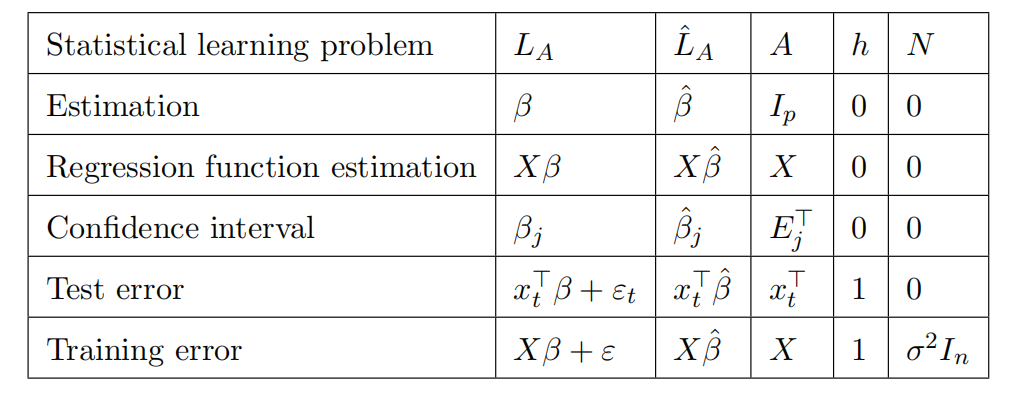
\includegraphics[width=1\textwidth]{linear.png}
\end{figure}

对所有的评判标准,我们都采用$MSE$来评价回归效果:
\[
    M(\hat\beta_0) = \mathbb E {\Vert L_A - \hat L_A (\hat\beta_0) \Vert }^2,
\]  
并用一体式学习和分布式学习$MSE$的比值代替分布式学习的效率:
\[
    E(A;X_1,\ldots,X_k) := \frac{M(\hat \beta)}{M(\hat \beta_{dist})},
\]  
其中$A$代表评判标准,k代表分布的个数。

容易算出:
\[
    E(a,d;X_1,\ldots,X_k) = \frac{
        tr[{(X^T X)}^{-1}A^T A] - 2tr[{A(X^T X)}^{-1}X^T N] + hd
    }
    {
        \sum\limits_{i=1}^k w_i^2 \cdot tr[{(X_i^T X_i)}^{-1}A^T A] -2w_i \cdot tr[A{(X_i^T X_i)}^{-1}X_i^T N_i] + hd
    }.
\] 

利用$f(X) = \frac{1}{tr(X^{-1}A^T A)}$是定义在正定矩阵上的凹函数这一点,可以求出最优权重为:
\[
    w_i= \frac{\lambda^* + b_i}{a_i},
\]  
其中$a_i=tr[{(X_i^T X_i)}^{-1}A^T A], \; b_i = tr[A{(X_i^T X_i)}^{-1}X_i^T N_i], \; \lambda^* = \frac{
    1-\sum\limits_{i=1}^k\frac{b_i}{a_i}
}{
    \sum\limits_{i=1}^k\frac{1}{a_i}
}$ 。

注意到最终的表达式中出现了$X^T X$形式的矩阵。如果我们将样本视为轻尾分布的随机变量,我们是可以利用MP分布律及其变式求出$a_i,b_i$在
$n,p$按一定比例趋于无穷时的极限值。再通过计算在不同评判标准$A$下学习效率$E(A;X_1,\ldots,X_k)$关于分布数$k$的变化规律,我们就可以量化
地评价分布式学习对线性回归效率的影响程度了。

\subsection{核方法中的随机矩阵}

考虑一个k类高斯混合模型,即样本矩阵为$X = [x_1,\ldots,x_n] \in \mathbb R^{p\times n}$,且样本服从以下分布:
\[
    \begin{aligned}
        &x_1,\ldots,x_{n_1} && \sim \mathcal{N} (\mu_1,C_1)\\
        &\qquad\vdots && \qquad\quad\vdots \\
        &x_{n-n_k+1},\ldots,x_{n} && \sim \mathcal{N} (\mu_k,C_k)\\
    \end{aligned}
\]  
即样本由$k$种不同的正态分布样本($\mathcal{C}_1,\ldots,\mathcal{C}_k$)组成,其中$\mu_i \in \mathbb R ^p, C_i \in \mathbb R^{p\times p}$。由概率论知识,实际上如果$x_i \in \mathcal{C}_a$,则
$x_i = \mu_a + C_a^{\frac{1}{2}}z_i$,其中随机变量$z_i$服从$p$维标准正态分布。

下面考虑样本的核矩阵:
\[
    K = {\{ f(\frac{1}{p}{\Vert x_i-x_j \Vert}^2) \}}_{i,j=1}^n,
\]  
其中$f$是一个足够光滑的函数,例如高斯核。我们将要用随机矩阵的理论证明核方法在分类问题上的有效性。

我们只看一个最简单的情形,即$C_1 = C_2 = \cdots = C_k = I_p$。
这种情况下$f$只用取$id$即可。注意到:
\[
    \frac{1}{p}{\Vert x_i-x_j \Vert}^2 = \frac{1}{p}{\Vert \mu_a-\mu_b \Vert}^2 +
    \frac{2}{p}{(\mu_a-\mu_b)}^T(z_i-z_j) + \frac{1}{p}{\Vert z_i \Vert}^2 + 
    \frac{1}{p}{\Vert z_j \Vert}^2 -\frac{2}{p} z_i^T z_j.
\]  

如果$\Vert \mu_a \Vert = O(\sqrt{p})$,则上式右侧中占主导数量级的项是$\frac{1}{p}{\Vert \mu_a-\mu_b \Vert}^2 + 2$,其中2是两个
$\frac{1}{p}{\Vert z_i \Vert}^2 = 1+O(p^{-\frac{1}{2}})$产生的,其他项都是$O(p^{-\frac{1}{2}})$量级的。这也就是说,从核矩阵的每一个元素来看,
占主导的项就是样本所属类别的差异。

但如果我们只能保证$\Vert \mu_a-\mu_b \Vert = O(1)$,此时上式中的主导项(除了2之外)就变成了包含随机元素的
$\frac{2}{p} z_i^T z_j$,即从每个元素来看,似乎核矩阵并不能反映出样本的区别。

这时就需要从随机矩阵整体的角度去分析这个问题。下面我们将用矩阵和向量的形式将核矩阵拆分开来:
\[
    \begin{aligned}
        {\{\frac{1}{p}{\Vert x_i-x_j \Vert}^2\}}_{i,j=1}^n = &
         2 \cdot 1_n 1_n^T + \frac{1}{p}J{\{{\Vert \mu_a-\mu_b \Vert}^2\}}_{a,b=1}^k J^T \\
        & + \psi 1_n^T + 1_n \psi^T - \frac{2}{p}Z^T Z + \frac{2}{p}(d 1_n^T + 1_n d^T) \\
        & -\frac{2}{p}(J M^T Z + z^T M J^T) - diag(\cdot), \\
    \end{aligned}
\]
其中$J$为扩充矩阵,即$J=[j_1,\ldots,j_k] \in \mathbb R ^{n\times k}$,$j_a$ 为只在第$n_1+\cdots+n_{a-1}+1$到第$n_1+\cdots+n_a$项为1其余项均为0的列向量,$M = [\mu_1,\ldots,\mu_k] \in \mathbb R ^{p \times k}$,$\psi \in \mathbb R ^n$且它的每个元素为$1-\frac{{\Vert z_i \Vert}^2}{p}$,$d = diag(JM^T Z)\in \mathbb R^n$,$-diag(\cdot)$是去除对角元素的操作。

通过考察上式右侧各项(在矩阵范数意义下的)数量级,我们发现此时包含$\mu_a-\mu_b$的关键信息项和白噪声项$\frac{2}{p}Z^T Z$
为同一数量级,均为$O(1)$。但在逐元素的分析中噪声项是会盖过关键信息项的,这也体现了从整体去分析问题的优势。

出现这种情况可以这样理解:关键信息矩阵的秩不高,所以能量的聚集会更加集中。

事实上,所有量级为$O(1)$的项为:
\[
    -\frac{2}{p}Z^T Z + \frac{1}{p}J{\{{\Vert \mu_a-\mu_b \Vert}^2\}}_{a,b=1}^k J^T + \frac{2}{p}(d 1_n^T + 1_n d^T)
    - \frac{2}{p}(J M^T Z + z^T M J^T),
\]  
这是一个典型的Spiked模型——后面三项可以看成一个至多秩为$2k+2$的矩阵。所以接下来我们就可以通过Spiked模型中扰动和阈值$c$的关系,
进一步分析什么时候扰动(关键信息)可以从杂乱的随机白噪声中凸显出来。

\bibliographystyle{unsrt}
\bibliography{ref}

\end{document}
